\section [Serial and Parallel Reactions (1D)]{1D reactive transport: multispecies transport with serial and parallel reactions }
\label{benchmark_1d_chain_reaction}

Reaction networks can be classified as serial and/or parallel reaction networks. Serial reaction is a reactant produces a single product and this product becomes the reactant for the next stage producing another single product. Examples of serial reactions can be denitrification, radioactive decay and dechlorination of some chlorinated solvents. In parallel reactions,  the parent reactant undergoes two or more independent reactions to produce multiple products. In many biogeochemical systems, the reaction networks are the combination of serial and parallel reactions. 

\subsection{Definition}

In scenario 1, sequential reductive dechlorination of chlorinated hydrocarbons from trichlorobenzene (TCB) to diclorobenzene (DCB) to monochlorobenzene (MCB) is simulated:
\begin{equation}
TCB \rightarrow DCB \rightarrow MCB
\end{equation}
In scenario 2, a serial-parallel reaction network as shown in Fig.~\ref{chain_reactions} is used to perform the verification. It can be decomposed into three serial reactions: $A \rightarrow B \rightarrow C_1, A \rightarrow B \rightarrow C_2, A \rightarrow B \rightarrow C_3$. For all the reactions in this scenario, first-order irreversible reactions are assumed. 

An analytical solution by \cite{Sun:1999} has been used to verify the numerical results from OpenGeoSys-BRNS simulation for these two scenarios. 

\begin{figure}[htbp]
\centering
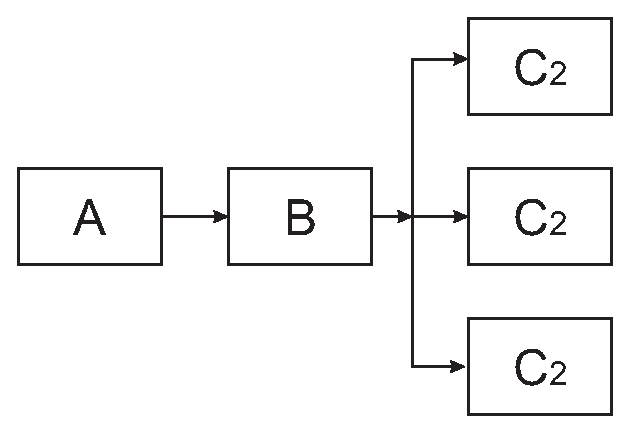
\includegraphics[width=0.6\textwidth]{PART_III/HC/Chain_Reaction_Figure1_Serial_Pararrel_Reactions.eps}
\caption{An example of serial-parallel reaction network. }
\label{chain_reactions}
\end{figure}

In scenario 1, a sand column of 100 meters length is flushed constantly by water containing TCB. The microbial groups in the column then start to convert TCB to DCB and further to product MCB. In OGS-BRNS model, a line of 100 meters with spatial discretization of 2 meters is defined. Water flows from left to right with velocity of 20 m/d. The dispersivity is 5 meters. The first order reaction rates of TCB, DCB and MCB are 0.0013, 0.00024, 0.00019 1/d respectively. The yield factor from TCB to DCB is 0.81 and from DCB to MCB is 0.765. The total simulation time is 1.5 days and temporal discretization of 0.01 day is employed. The initial and boundary conditions are
~~\\
For $x \geq 0$,

\begin{equation}
c_{TCB}(x,0) = c_{DCB}(x,0) = c_{MCB}(x,0) = 0  \\
\end{equation}
For $t > 0$, 
\begin{equation}
c_{TCB}(0,t)=10.0 \\
c_{DCB}(0,t)=c_{MCB}(0,t)=0   \\
c_{TCB}(\infty,t)=c_{DCB}(\infty,t)=c_{MCB}(\infty,t)=0   \\
\end{equation}

Scenario 2 has similar numerical settings but with different parameter values. The column length is 40 meters with spatial discretization of 1 meter. Water flow velocity is 0.4 m/d. The dispersivity is 10 meters. The total simulation time is 40 days with temporal discretization of 0.04 day. The first order reaction rates and yield factors of the five species are listed in Table~\ref{tab:chain_reaction_param}. 
~~\\
For $x \geq 0$, 
\begin{equation}
c_{A}(x,0)=c_{B}(x,0) = c_{C_1}(x,0) = c_{C_2}(x,0) = c_{C_3}(x,0)   \\
\end{equation}
For $t > 0$, 
\begin{equation}
c_{A}(0,t) =1.0, 
\end{equation}
\begin{equation}
c_{B}(0,t) = c_{C1}(0,t) = c_{C_2}(0,t) = c_{C_3}(0,t)=0  
\end{equation}
\begin{equation}
c_{A}(\infty,t) = c_{B}(\infty,t)=c_{C_1}(\infty,t)= c_{C_2}(\infty,t)= c_{C_3}(\infty,t)=0   \\
\end{equation}

\begin{table}[!th]
\begin{center}
\begin{tabular}{lrl}
\hline\noalign{\smallskip}
Parameter & Value & Unit \\
\hline\noalign{\smallskip}
% JT-> someone.  there is a problem here.   \codt perhaps not defined???
%Reaction rate of A         &   0.2  &  $1 \codt d^{-1}$ \\
%Reaction rate of B         &   0.1  &  $1 \codt d^{-1}$ \\
%Reaction rate of C1        &   0.02 &  $1 \codt d^{-1}$ \\
%Reaction rate of C2        &   0.02 &  $1 \codt d^{-1}$ \\
%Reaction rate of C3        &   0.02 &  $1 \codt d^{-1}$ \\
%Yield factor from A to B   &   0.5  &   -    \\
%Yield factor from B to C1  &   0.3  &   -    \\
%Yield factor from B to C2  &   0.2  &   -    \\
%Yield factor from B to C3  &   0.1  &   -    \\
\noalign{\smallskip}\hline
\end{tabular}
\end{center}
\caption{Values of first order reaction rates and yield factors for scenario 2.} 
\label{tab:chain_reaction_param}
\end{table}

\subsection{Solution}
The comparison was conducted for the concentration of all the species for scenario 1 and 2. Fig.~\ref{chain_reactions_fig2} shows a very good agreement between analytical and numerical results for scenario 1.  For scenario 2, as we can see from Fig.~\ref{chain_reactions_fig3} and~\ref{chain_reactions_fig4}, the results obtained from OGS-BRNS also fit well with analytical solution.

\begin{figure}[htbp]
\centering
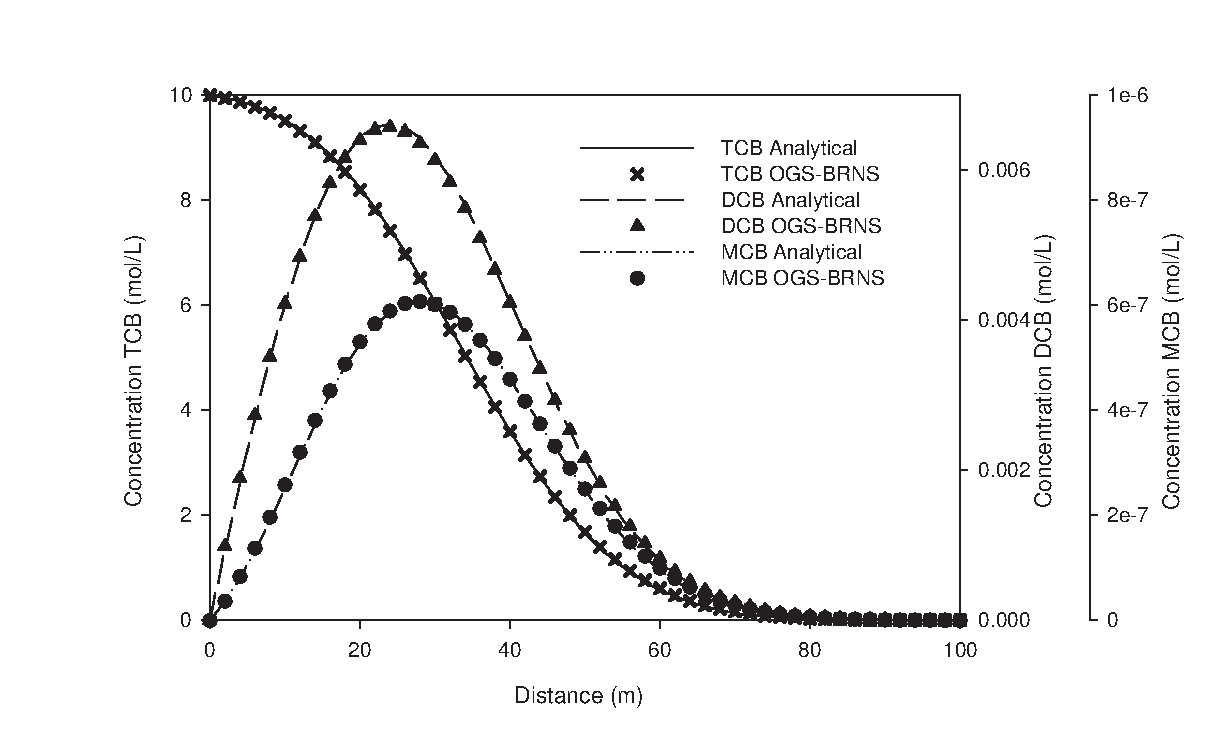
\includegraphics[width=0.6\textwidth]{PART_III/HC/Chain_Reaction_Figure2_TCBdegradation3.eps}
\caption{Comparison between concentration profiles of TCB, DCB and MCB calculated by analytical solution and \GeoSys-BRNS in scenario 1. }
\label{chain_reactions_fig2}
\end{figure}

\begin{figure}[htbp]
\centering
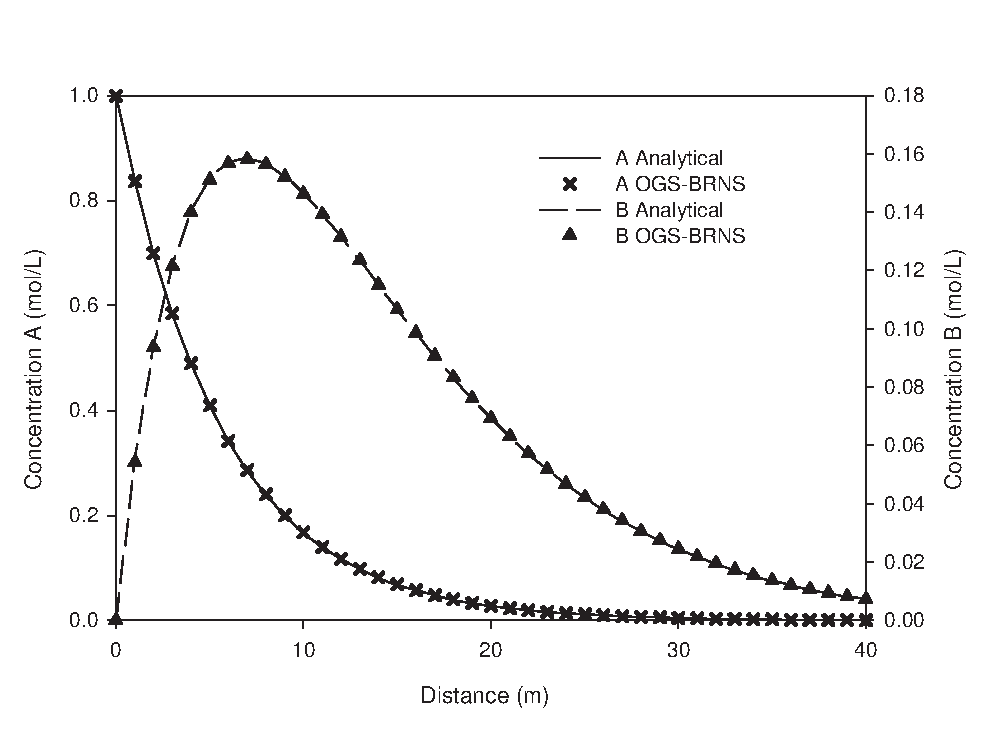
\includegraphics[width=0.6\textwidth]{PART_III/HC/Chain_Reaction_Figure3_sun1999verification2_AB.eps}
\caption{Comparison between concentration profiles of species A and B calculated by analytical solution and \GeoSys-BRNS in scenario 2. }
\label{chain_reactions_fig3}
\end{figure}

\begin{figure}[htbp]
\centering
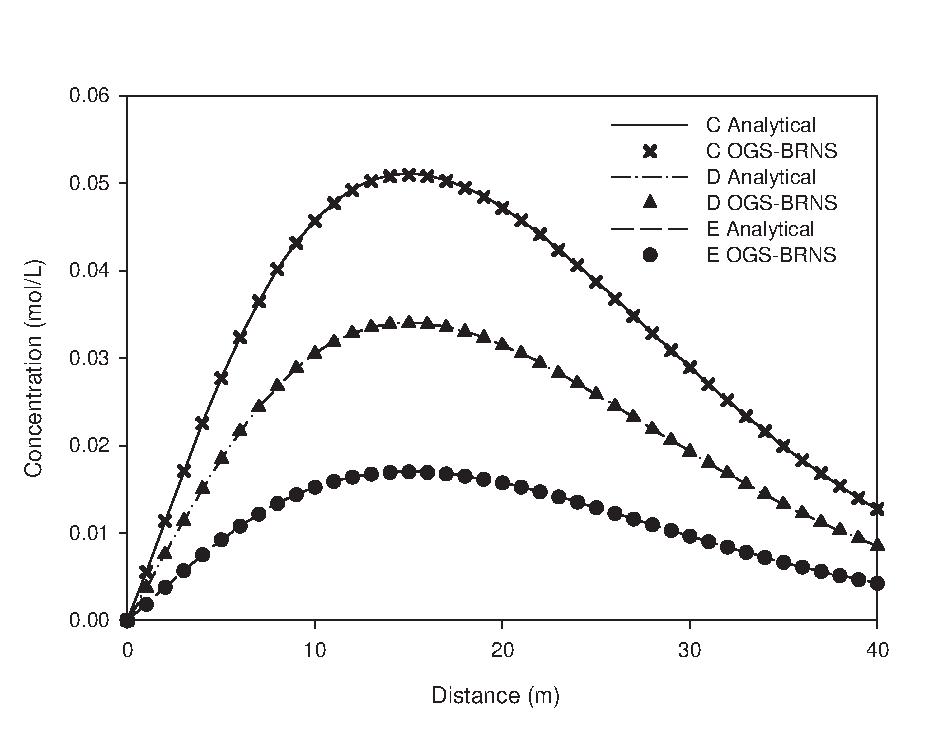
\includegraphics[width=0.6\textwidth]{PART_III/HC/Chain_Reaction_Figure4_sun1999verification2_CDE.eps}
\caption{Comparison between concentration profiles of species C, D and E calculated by analytical solution and \GeoSys-BRNS in scenario 2. }
\label{chain_reactions_fig4}
\end{figure}

